\section{Collecte des données et analyse des résultats}

\subsection{Présentation des données et analyse des résultats}

\subsubsection{Analyse descriptive.}
\par{Encore appelé statistique descriptive, l'analyse descriptive
    permet de décrire et de résumer les caractéristique essentielles d'un ensemble de données.
    En analyse technique, en plus des statistiques élémentaire on peut faire 
    également une analyse des tendances 
    pour comprendre les mouvements de prix d'un actif financier au fil du temps.
    De  plus une analyse des niveaux de résistances et de support permet de fournir 
    des repères pour déterminer les
    zones ou les prix sont susceptible de réagir ou potentiellement inverser leur direction.}

\begin{itemize}
    \item[$\diamondsuit$]\textbf{L'indice BRVM-Services-Publics.}    
    \par{L'analyse descriptive des données de la BRVM-Agriculture, basée sur les données 
        antérieures de la Bourse régionale des valeurs immobilières sur la période allant du 
        \textbf{16 juin 2020} au \textbf{15 mai 2023}, révèle de nombreux points importants.
        En effet, la valeur moyenne de cet indice durant cette période s'élève à 439,55, ce qui 
        indique un niveau de prix autour duquel les prix tendent à se regrouper. L'écart type 
        de 47,60 suggère que les prix de clôture sont légèrement dispersés par rapport à la moyenne, 
        ce qui explique une certaine stabilité dans les fluctuations. Le prix minimum atteint durant 
        cette période est de 328,64 tandis que le prix maximum atteint est de 528,59. En étudiant les quartiles,
        nous pouvons remarquer que 25\% des prix sont inférieurs à 397,54, tandis que 75\% des prix de clôture
        sont inférieurs à 475,15, ce qui montre une distribution des prix légèrement asymétrique. 
        Avec une valeur de 449,34, la médiane indique que la moitié des prix sont inférieurs à cette valeur.
        Suivant les niveaux de résistance et de support sur la figure ci-dessous, nous pouvons remarquer qu'aucune ligne
        de support ni de résistance ne respecte la "règle des trois touches", qui suggère que la résistance et le 
        support sont valides lorsqu'ils ont été touchés au moins trois fois sans être traversés 
        par la courbe des prix.}
        \par{
        En général, nous pouvons noter une légère augmentation du cours de l'indice durant la période
        allant de juin 2020 à mai 2023. Cette augmentation traduit une appréciation positive de la valeur
        par les investisseurs ou simplement une demande de plus en plus importante pour cette valeur.}
        
        \begin{figure}[h]
            \centering
            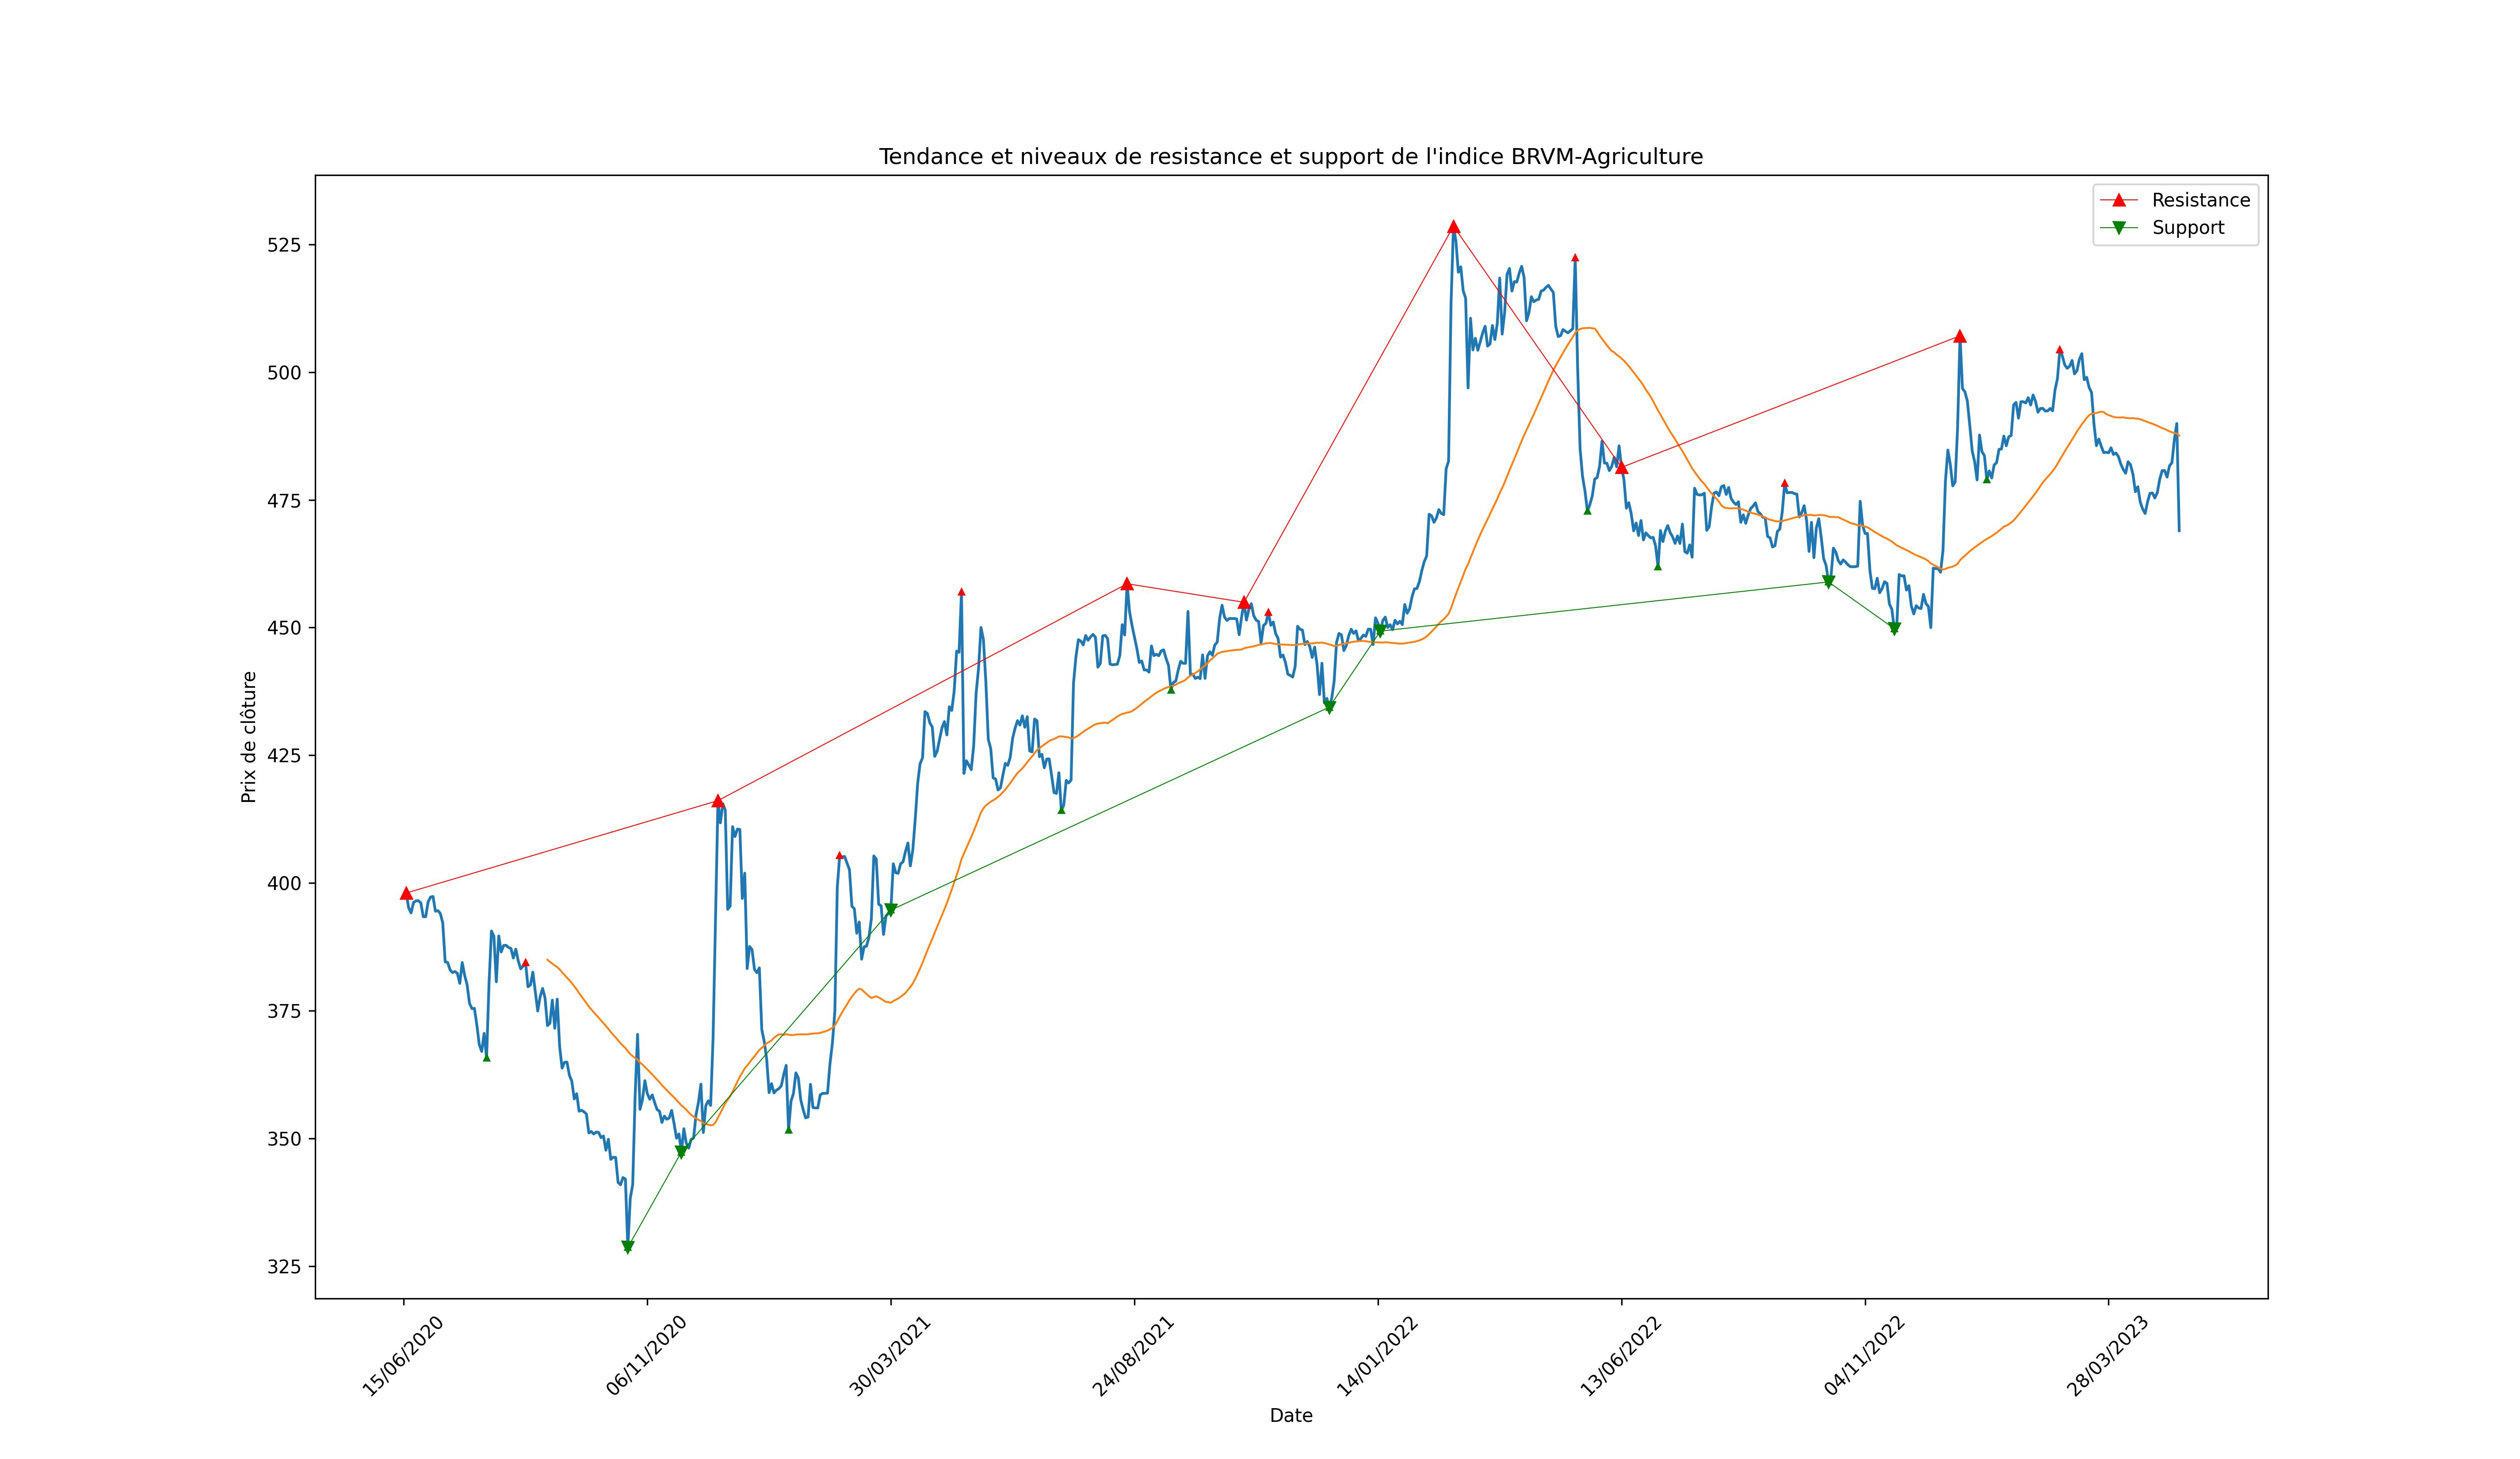
\includegraphics[width=1 \textwidth ]{img/public_tendance.jpg}
            \caption{Tendances de l'indice BRVM-Services-Publics}
            \label{fig:Tendances de l'indice BRVM-Services-Publics}
          \end{figure}

    \item[$\diamondsuit$] \textbf{BRVM-Agriculture}
    \par{L'analyse descriptive de l'indice BRVM-Agriculture sur la période du \textbf{16 juin 2020} au
        \textbf{15 mai 2023} révèle principalement une très grande augmentation du cours de la valeur.
        En effet, à la date du 15 mai 2023, le prix de l'indice BRVM-Agriculture valait 65,92 pour atteindre
        248,05 Fcfa le 15 mai 2023. Autrement dit, la valeur vaut plus de 3,5 fois sa valeur initiale. 
        Par ailleurs, le prix minimum atteint durant cette période est de 55,40 Fcfa enregistré le
        \textbf{mercredi 05 août 2020} et un maximum de 349,65 Fcfa atteint le \textbf{lundi 16 mai 2022}.
        En moyenne, le prix de clôture de la "BRVM-Agri" durant cette période tourne autour de 206,82 Fcfa.
        L'étude des quartiles révèle que 25\% des cours sont inférieurs à 109,59 Fcfa et 75\% sont 
        inférieurs à 287,00 Fcfa. En plus d'un écart type de 95,12, qui suggère une légère 
        distribution par rapport à la moyenne, nous pouvons remarquer graphiquement une évolution des cours 
        très progressive et sans changement brusque.
        Suivant les niveaux de résistance et de support, nous pouvons remarquer que seulement la troisième 
        résistance ne respecte pas la "règle des trois points touchés".
        En effet, nous pouvons observer que la résistance qui commence vers le 09 novembre 2020 
        est touchée cinq fois par la courbe de l'évolution des cours de la valeur avant d'être traversée
        plutôt au sixième pic vers le 25 août 2022 pour atteindre un nouveau record de 259,08 Fcfa le
        \textbf{mardi 26 octobre 2021}, ce qui valide la résistance précédente.}

        \begin{figure}[h]
            \centering
            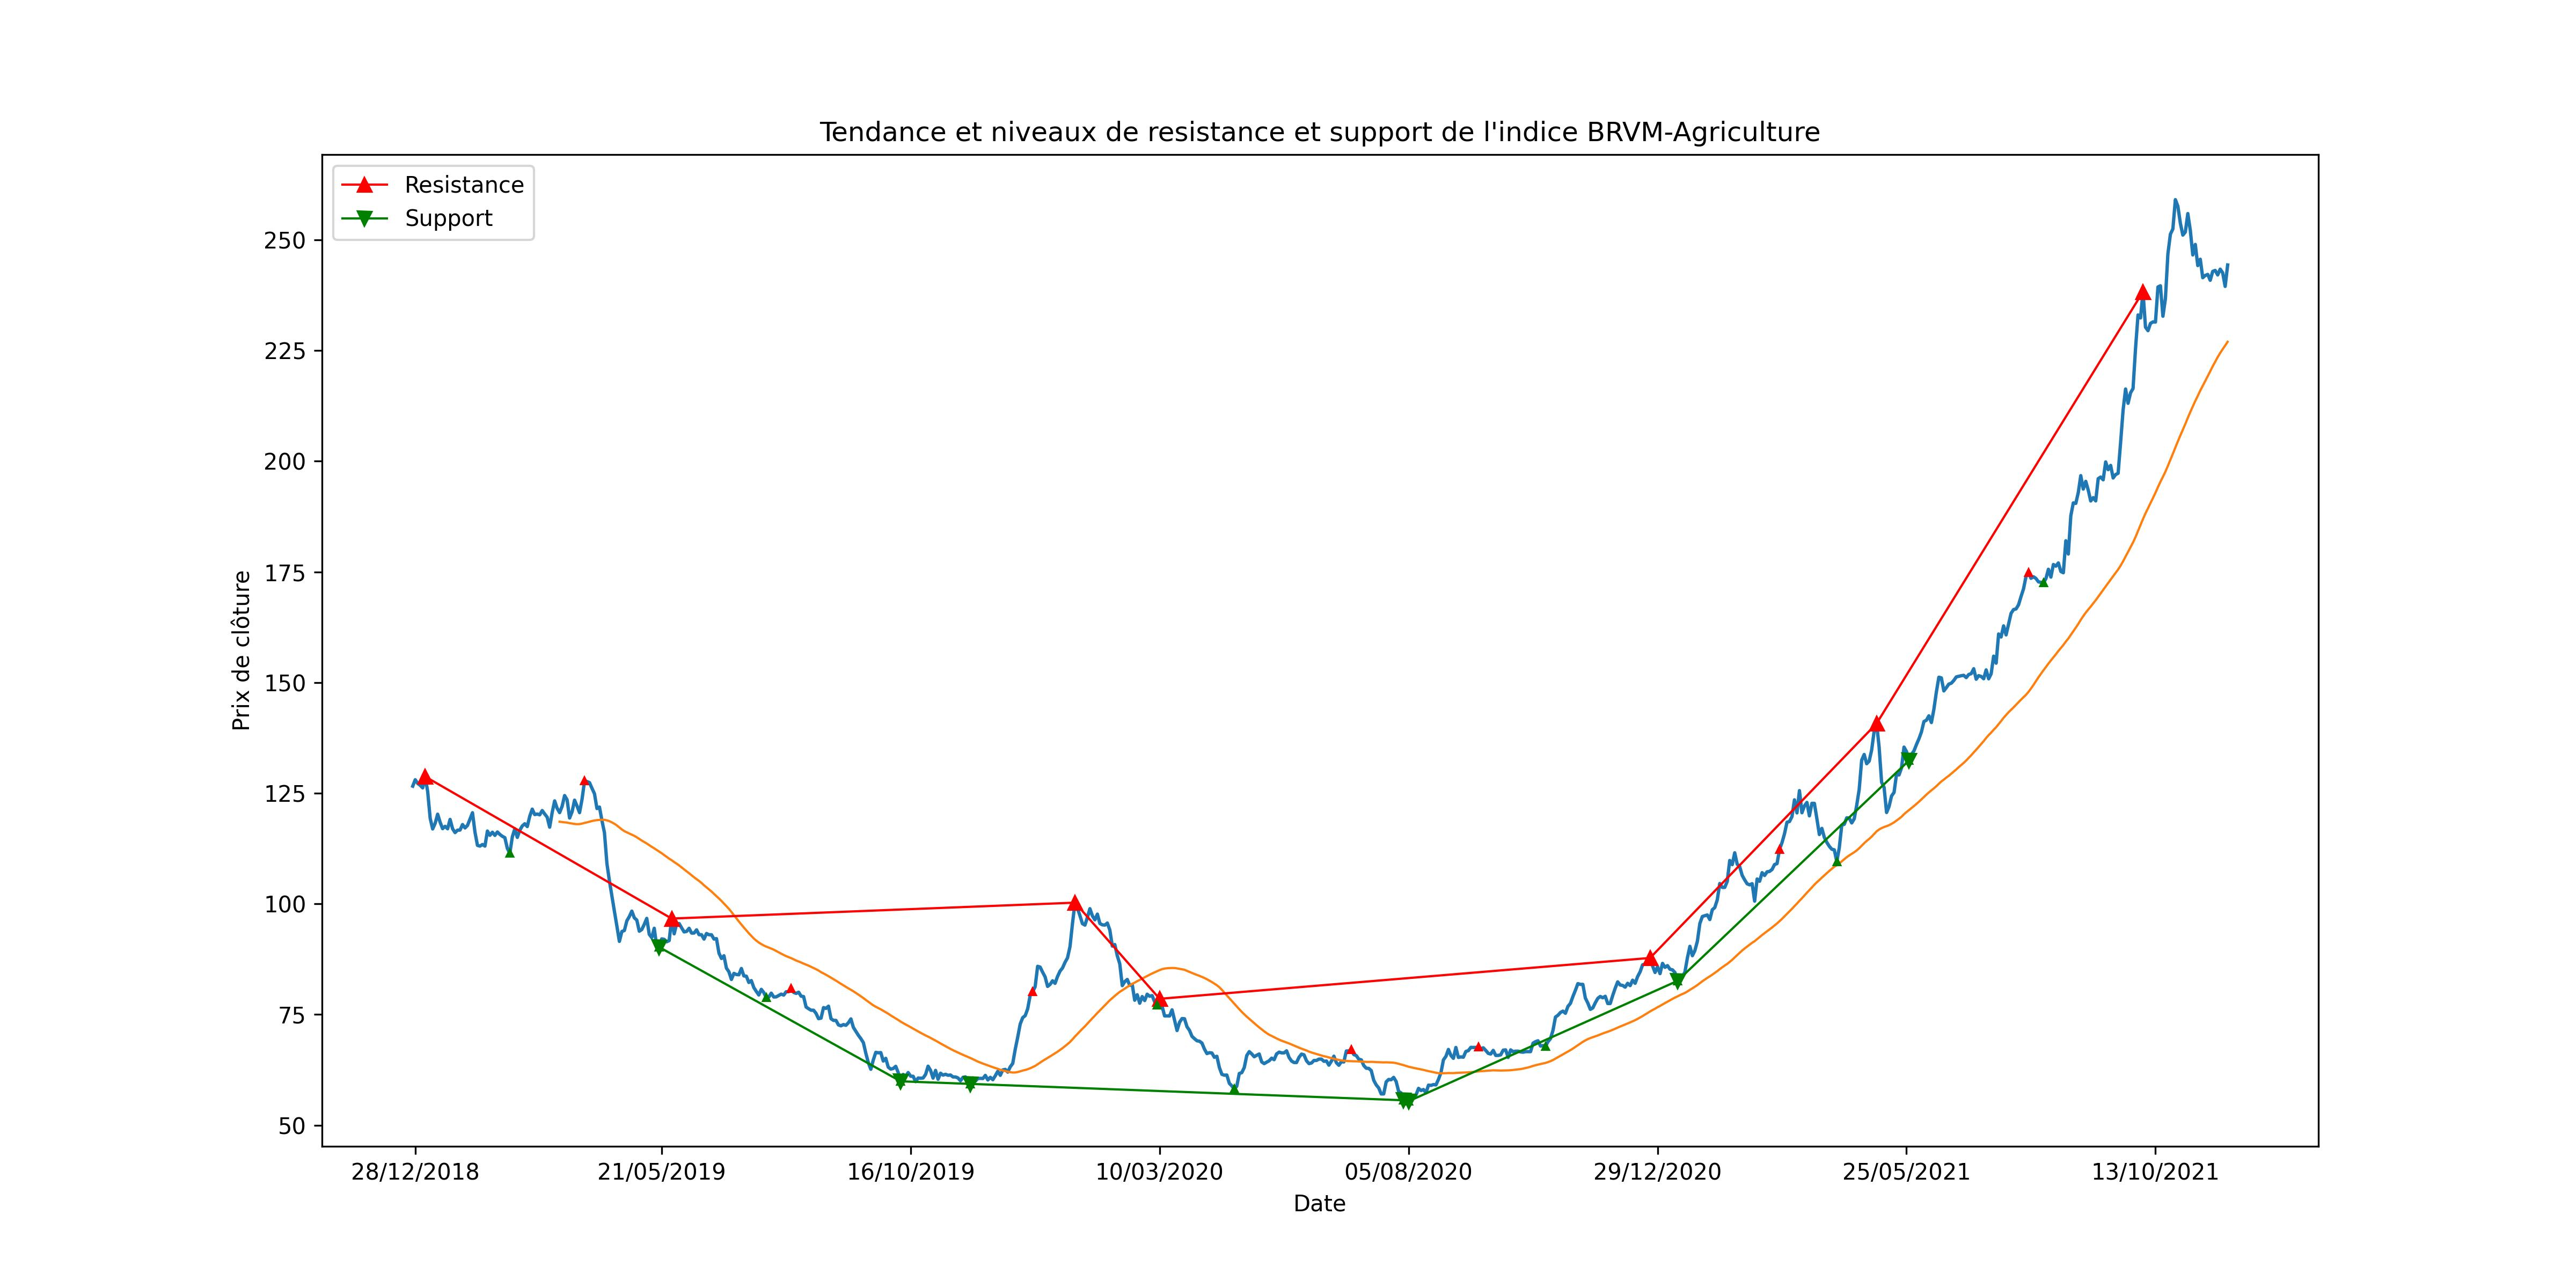
\includegraphics[width=1 \textwidth ]{img/agri_tendance.jpg}
            \caption{Tendances de l'indice BRVM-Agriculture}
            \label{fig:Tendance de l'indice BRVM-Agriculture}
        \end{figure}
\end{itemize}



